\documentclass{article}

\usepackage[
  paperheight=8.5in,
  paperwidth=5.5in,
  left=10mm,
  right=10mm,
  top=20mm,
  bottom=20mm]{geometry}
\usepackage[utf8]{inputenc}

\usepackage{graphicx}
\usepackage{wrapfig}
\usepackage[bottom]{footmisc}
\usepackage{listings}
\usepackage{enumitem}

\usepackage{wrapfig}
\usepackage{ragged2e}

\usepackage{array}
\usepackage[table]{xcolor}
\usepackage{multirow}
\usepackage{booktabs}
\usepackage{hhline}
\definecolor{palegreen}{rgb}{0.6,0.98,0.6}

\usepackage{amsmath}
\usepackage{amssymb}
\usepackage{multicol}
\usepackage{lipsum}
\usepackage{hyphenat}
\PassOptionsToPackage{hyphens}{url}
\usepackage{url}

\usepackage{rotating}

\usepackage{xeCJK}

%% support use of straight quotes in code listings
\usepackage[T1]{fontenc}
\usepackage{textcomp}
\usepackage{listings}
\lstset{upquote=true}

%% for shrinking space between lines
\usepackage{setspace}

\newcommand*{\affaddr}[1]{#1} % No op here. Customize it for different styles.
\newcommand*{\affmark}[1][*]{\textsuperscript{#1}}
\newcommand*{\email}[1]{\small{\texttt{#1}}}
\newcommand{\tarot}{\textsc{Tarot}}
\renewcommand*\contentsname{\centering Table of Contents}

\renewcommand{\footnoterule}{%
  \kern -3pt
  \hrule width \textwidth height 0.5pt
  \kern 2pt
}

% remove date
\date{}

\usepackage{titlesec}
\titleformat*{\section}{\large\bfseries}
\titleformat*{\subsection}{\normalsize\bfseries}
\titleformat*{\subsubsection}{\normalsize\bfseries}


\title{Manuscript Formatting Instructions\footnote{\protectCopyright \copyright 2022 by the Consortium for Computing Sciences in Colleges.
Permission to copy without fee all or part of this material is granted provided
that the copies are not made or distributed for direct commercial advantage,
the CCSC copyright notice and the title of the publication and its date appear,
and notice is given that copying is by permission of the Consortium for
Computing Sciences in Colleges.  To copy otherwise, or to republish, requires
a fee and/or specific permission.
}
}

% Target typesetting:
%
%  Baochuan Lu, Author A, John Meinke, Author B
%        Computer and Information Sciences
%          Southwest Baptist University
%               Bolivar, MO 65613
%            {blu,author}@sbuniv.edu
%          Computer Science Department
%              Another University
%              Our Town, TX 00000
%           {jmeinke,author}@univ.edu

\author{
Baochuan Lu\affmark[1], Author A\affmark[1], John Meinke\affmark[2], Author B\affmark[2]\\
\affaddr{\affmark[1]Computer and Information Sciences}\\
\affaddr{Southwest Baptist University}\\
\affaddr{Bolivar, MO 65613}\\
\email{\{blu,author\}@sbuniv.edu}\\
\affaddr{\affmark[2]Computer Science Department}\\
\affaddr{Another University}\\
\affaddr{Our Town, TX 00000}\\
\email{\{jmeinke,author\}@univ.edu}\\
}

\begin{document}
\maketitle

\begin{abstract}
This document describes manuscript formatting requirements for CCSC conferences. Authors can use this document as a template to format their papers.
\end{abstract}

\section{Length}
Prepare the paper for written understanding with a length of approximately six (6) single-spaced pages including tables, figures, and a list of references or bibliography.

\section{Style}
Write clearly and simply in the third person for an audience that is well-grounded in computing, but who may have limited exposure or knowledge about the specific topic of your paper. Define any technical terms deemed to require clarification when they are introduced.

\section{Title and Author Information}
Please follow the example in this paper to enter title and author information.

\section{Body of the Manuscript}
The text may be organized into sections and subsections. Please use \verb+\section+ and  \verb+\subsection+ commands to define them as shown in this paper. Latex will apply section formatting rules. If you opt to number your sections and subsections, do so specifically using Arabic numbers.

\subsection{Abstract}
Provide a one-paragraph brief overview of the paper in both the manuscript for review and in the final manuscript for publication.

\subsection{Citation}
Appropriately cite all references to other published works included in the paper. \texttt{biblatex} is used to create a list of references or bibliography as the last section in the paper. Here are citation examples for a book\cite{latexcompanion}, a journal paper\cite{einstein}, a website\cite{knuthwebsite}, and a conference proceeding paper\cite{maurer}.

\subsection{Lists}
Lists are easy to create in  \LaTeX\ whether they are ordered, unordered, or nested as shown in the following example.

\begin{itemize}[noitemsep]
  \item The individual entries are indicated with a black dot, a so-called bullet.
  \item The text in the entries may be of any length.
\end{itemize}

\begin{enumerate}[noitemsep]
  \item The labels consist of sequential numbers.
  \item The numbers start at 1 with every call to the enumerate environment.
\end{enumerate}

\begin{enumerate}[noitemsep]
   \item The labels consists of sequential numbers.
   \begin{itemize}[noitemsep]
     \item The individual entries are indicated with a black dot, a so-called bullet.
     \item The text in the entries may be of any length.
   \end{itemize}
   \item The numbers start at 1 with every call to the enumerate environment.
\end{enumerate}

\subsection{Math Expressions}
The mass-energy equivalence is described by the famous equation

$$E=mc^2$$

discovered in 1905 by Albert Einstein.
In natural units ($c$ = 1), the formula expresses the identity

\begin{equation}
E=m
\end{equation}

\subsection{Tables and Figures}
Include all tables and figures within the body of the text. (Provide as separate files in the original format any figures so that if there are problems with the figures coming into the final manuscript there are alternatives available to the editors.)

Here is an example Table \ref{table:nonlin}.

\begin{table}[ht]
\caption{Nonlinear Model Results} % title of Table
\label{table:nonlin} % is used to refer this table in the text
\centering % used for centering table
\begin{tabular}{c c c c} % centered columns (4 columns)
\hline\hline %inserts double horizontal lines
Case & Method\#1 & Method\#2 & Method\#3 \\ [0.5ex] % inserts table
%heading
\hline % inserts single horizontal line
1 & 50 & 837 & 970 \\ % inserting body of the table
2 & 47 & 877 & 230 \\
3 & 31 & 25 & 415 \\
4 & 35 & 144 & 2356 \\
5 & 45 & 300 & 556 \\ [1ex] % [1ex] adds vertical space
\hline %inserts single line
\end{tabular}
\end{table}

Here is an example Figure \ref{figure:universe}.

\begin{figure}[h!]
\centering
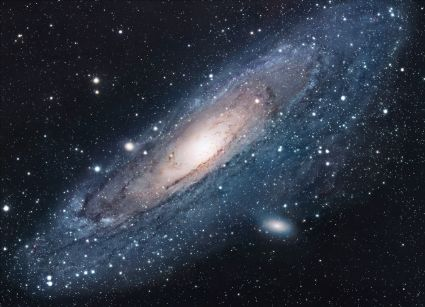
\includegraphics[scale=1.7]{universe}
\caption{The Universe}
\label{figure:universe}
\end{figure}

\subsection{Reference List}
The \verb+\printbibliography+ command prints a list of referneces for you. Please use \texttt{sample.bib} as an example to create your bibliography entries.

\subsection{Code Listings}
Commands from \texttt{listings} package allow you to display code easily with customizable coloring and styling rules. Here is an example.

\begin{lstlisting}[language=Python,  caption=Python example]
x = 42
epsilon = 0.01
step = epsilon**2
num_guesses = 0
ans = 0.0
while abs(ans**2-x) > epsilon and ans < x:
    ans = ans + step
    num_guesses += 1
if abs(ans**2-x) <= epsilon:
    print(str(ans) +
    ' is close to the square root of ' +
    str(x))
else:
    print('Failed to find square root of ' + str(x))
print("The number of guesses is " + str(num_guesses))
\end{lstlisting}

\section{Manuscript Submission}
The following materials will need to be submitted:
\begin{enumerate}[noitemsep]
  \item The final manuscript in Latex.
  \item Copyright release. It is essential that we receive the copyright release form. By signing this form you are acknowledging that the manuscript has not been printed in another venue, plus you are retaining your rights for use of the manuscript. Read the copyright release. The Consortium will not prohibit you from using the manuscript, but will ask that you credit any reuse to the Consortium as the original source of publication. If you misplace the copyright form, a generic copyright form can be found through the Copyright Release Form\cite{copyright}.\\
  The Consortium encourages multiple presentations of tutorials and workshops. If you are presenting a tutorial or workshop you may retain the copyright, but we must have that documented. Keep in mind that your manuscript is limited to two pages total. However, you must still submit a copyright form.\\
  Please note that it is critical that you obtain permission to use third party material. If you use diagrams and such that are attributable to a third party you must obtain formal permission to reprint such items, and must so indicate in the copyright release as well as submit such permission.
  \item Registration for the conference, along with the appropriate registration fee. We have found that there are some folks in need of publication for promotion and tenure purposes, and then don’t want to present the paper. A major plus of the Consortium conferences is the presentation of the papers, and you must plan on attending. If you do not present the paper at the conference the paper will be removed from the ACM Digital Library.
  \item A statement of any special presentation needs that you may have.
  \item A pdf version of your manuscript is most helpful. If there are problems with special characters or special formatting this provides the editors with what you expected your final manuscript to look like. Providing a pdf version or a hard copy helps significantly in envisioning what the author expected the final product to look like.
  \item Electronic copies of any graphics in a standard format (bitmap, jpeg, tiff).
\end{enumerate}

\section{Additional Information}
Please feel free to email \verb+ccsc-editors@googlegroups.com+ for questions. This document is modified from the CCSC manuscript formatting document\cite{meinke} created by John Meinke.

\medskip

\bibliographystyle{plain}
\bibliography{sample}

\end{document}
